\documentclass[../../PS3.tex]{subfiles}

\definecolor{bggrey}{gray}{.9}


\begin{document}
\graphicspath{{images/}{./problems/Prob1/images/}}


% !TeX spellcheck = en_GB
\section{Sunlight}

We want to find the energy density per volume for blackbody radiation for given wavelength $\lambda$ and temperature $T$.

\subsection*{(a) $\rho(T, \lambda)$}

We can start with the expression for $U$ in terms of an integral over $k$:

\begin{equation}
	U = 2 \frac{V}{\left(2\pi\right)^3} 4 \pi \hbar c \int_0^\infty \dd{k} k^3 \left(e^{\beta \hbar c k} - 1\right)^{-1}
\end{equation}

We want this integral in terms of $\lambda$. We use $k = \frac{\tpi}{\lambda}$, and $\dd{k} = - \frac{\tpi}{\lambda^2} \dd{\lambda}$, to rewrite:

\begin{align}
	U &= 2 \frac{V}{\left(2\pi\right)^3} 4 \pi \hbar c \int_{k=0}^{k=\infty} \dd{k} \left(\frac{\tpi}{\lambda}\right)^3 \left(e^{ \frac{\beta \hbar c \tpi}{\lambda}} - 1\right)^{-1} \\
	U &=  2 \frac{V}{\left(2\pi\right)^3} 4 \pi \hbar c \int_{\lambda=\infty}^{\lambda = 0} \left(-\frac{\tpi}{\lambda^2}\right) \dd{\lambda} \left(\frac{\tpi}{\lambda}\right)^3 \left(e^{ \frac{\beta \hbar c \tpi}{\lambda}} - 1\right)^{-1} \\
	\frac{U}{V} &=   \frac{\tpi[4]}{\left(\pi\right)^3}  \pi \hbar c \int_{\lambda=\infty}^{\lambda = 0} \left(-\frac{1}{\lambda^2}\right) \dd{\lambda} \left(\frac{1}{\lambda}\right)^3 \left(e^{ \frac{\beta \hbar c \tpi}{\lambda}} - 1\right)^{-1} \\
	\frac{U}{V} &= \frac{\tpi[4]}{\pi^2}   \hbar c \int_{\lambda=\infty}^{\lambda = 0} \left(-\frac{1}{\lambda^2}\right) \dd{\lambda} \left(\frac{1}{\lambda}\right)^3 \left(e^{ \frac{\beta \hbar c \tpi}{\lambda}} - 1\right)^{-1} \\
	\frac{U}{V} &= - 16 \pi^2 \hbar c \int_{\lambda=\infty}^{\lambda = 0}  \dd{\lambda} \frac{1}{\lambda^5} \left(e^{ \frac{\beta \hbar c \tpi}{\lambda}} - 1\right)^{-1} \\
	\frac{U}{V} &= 16 \pi^2 \hbar c \int_{0}^{\infty}  \dd{\lambda} \frac{1}{\lambda^5} \left(e^{ \frac{\beta \hbar c \tpi}{\lambda}} - 1\right)^{-1}
\end{align}

We want the energy density per wavelength, so we can identify $\rho$ with the integrand:

\begin{equation}
	\rho(\lambda,\beta) = 16 \pi^2 \hbar c \frac{1}{\lambda^5} \left(e^{ \frac{\beta \hbar c \tpi}{\lambda}} - 1\right)^{-1}
\end{equation}

This means 

\begin{equation} \label{eq:P1:rhoans}
	\rho(\lambda,T) =  \frac{16 \pi^2 \hbar c}{\lambda^5} \left(e^{ \frac{\tpi \hbar c }{\kb T \lambda}} - 1\right)^{-1}
\end{equation}

\subsection*{(b) Finding $\lambda$ to maximise $\rho$}

Let's rewrite $\rho$ a bit:

\begin{equation}
	\rho(\lambda,T) =  \frac{16 \pi^2 \hbar c}{\lambda^5 \left(e^{ \frac{\tpi \hbar c }{\kb T \lambda}} - 1\right)}
\end{equation}

To simplify the math a bit, we can notice that maximising $\rho$ should be equivalent to minimising the denominator. Let's do that:

\begin{align}
	0 &= \dv{}{\lambda} \left( \lambda^5 \left(e^{ \frac{\tpi \hbar c }{\kb T \lambda}} - 1\right)\right) \\
	0 &= \lambda^5 \dv{}{\lambda} \left(e^{ \frac{\tpi \hbar c }{\kb T \lambda}} - 1\right) + \left(e^{ \frac{\tpi \hbar c }{\kb T \lambda}} - 1\right)\dv{}{\lambda} \lambda^5 
\end{align}

Continuing on, pausing only to admire symmetry,
\begin{align}
	- \lambda^5 \dv{}{\lambda} \left(e^{ \frac{\tpi \hbar c }{\kb T \lambda}} - 1\right) &= \left(e^{ \frac{\tpi \hbar c }{\kb T \lambda}} - 1\right)\dv{}{\lambda} \lambda^5 \\
	- \lambda^5 e^{ \frac{\tpi \hbar c }{\kb T \lambda}} \left( -\frac{\tpi \hbar c }{\kb T \lambda^2}\right) &= \left(e^{ \frac{\tpi \hbar c }{\kb T \lambda}} - 1\right)\left(5 \lambda^4\right) \\	
	\frac{\tpi \hbar c }{\kb T } \lambda^3 e^{ \frac{\tpi \hbar c }{\kb T \lambda}}  &= \left(e^{ \frac{\tpi \hbar c }{\kb T \lambda}} - 1\right)\left(5 \lambda^4\right)
\end{align}

Defining $y = \frac{\tpi \hbar c }{\kb T }$:

\begin{align}
	y e^{ \frac{y}{ \lambda}}  &= 5 \lambda \left(e^{ \frac{y}{\lambda}} - 1\right) \\
	\frac{y}{\lambda} &=  5 \left(1 - e^{-  \frac{y}{\lambda}}\right) 
\end{align}

I solved this for $\frac{y}{\lambda}$ in Mathematica, giving us two solutions. There's the pathological solution where $\frac{y}{\lambda} = 0$ This corresponds to $\lambda$ going to infinity. Looking back at \eqref{eq:P1:rhoans}, we may find ourselves more interested in the other solution, which we get to be $\frac{y}{\lambda} \approx 4.966$. We can solve this for $\lambda_{\mathrm{max}}$ for a given temperature:

\begin{align}
	\frac{y}{\lambda_{\mathrm{max}}} &= 4.966 \\
	\lambda_{\mathrm{max}} &= \frac{y}{4.966} \\
	\lambda_{\mathrm{max}} &= \frac{\tpi \hbar c }{4.966 \kb T } \label{eq:P1b:lambdamax}
\end{align}

\subsection*{(c) Solar temperature from $\lambda_\mathrm{max}$}

We're given here that $\lambda_\mathrm{max}$ for sunlight is $\SI{480}{\nano\meter}$, and we want to find the temperature of the radiation-emitting surface of the sun. We can solve \eqref{eq:P1b:lambdamax} for $T$: 

\begin{equation}
	T = \frac{\tpi \hbar c }{4.966 \kb \lambda_{\mathrm{max}} }
\end{equation}

I unnecessarily used Mathematica to solve for $T$, giving $T = \SI{6036}{K}$, which seems to be around the number I get when searching around.

\subsection*{(d) Differences between real spectrum and blackbody}


\begin{figure}[htp]
	\centering
	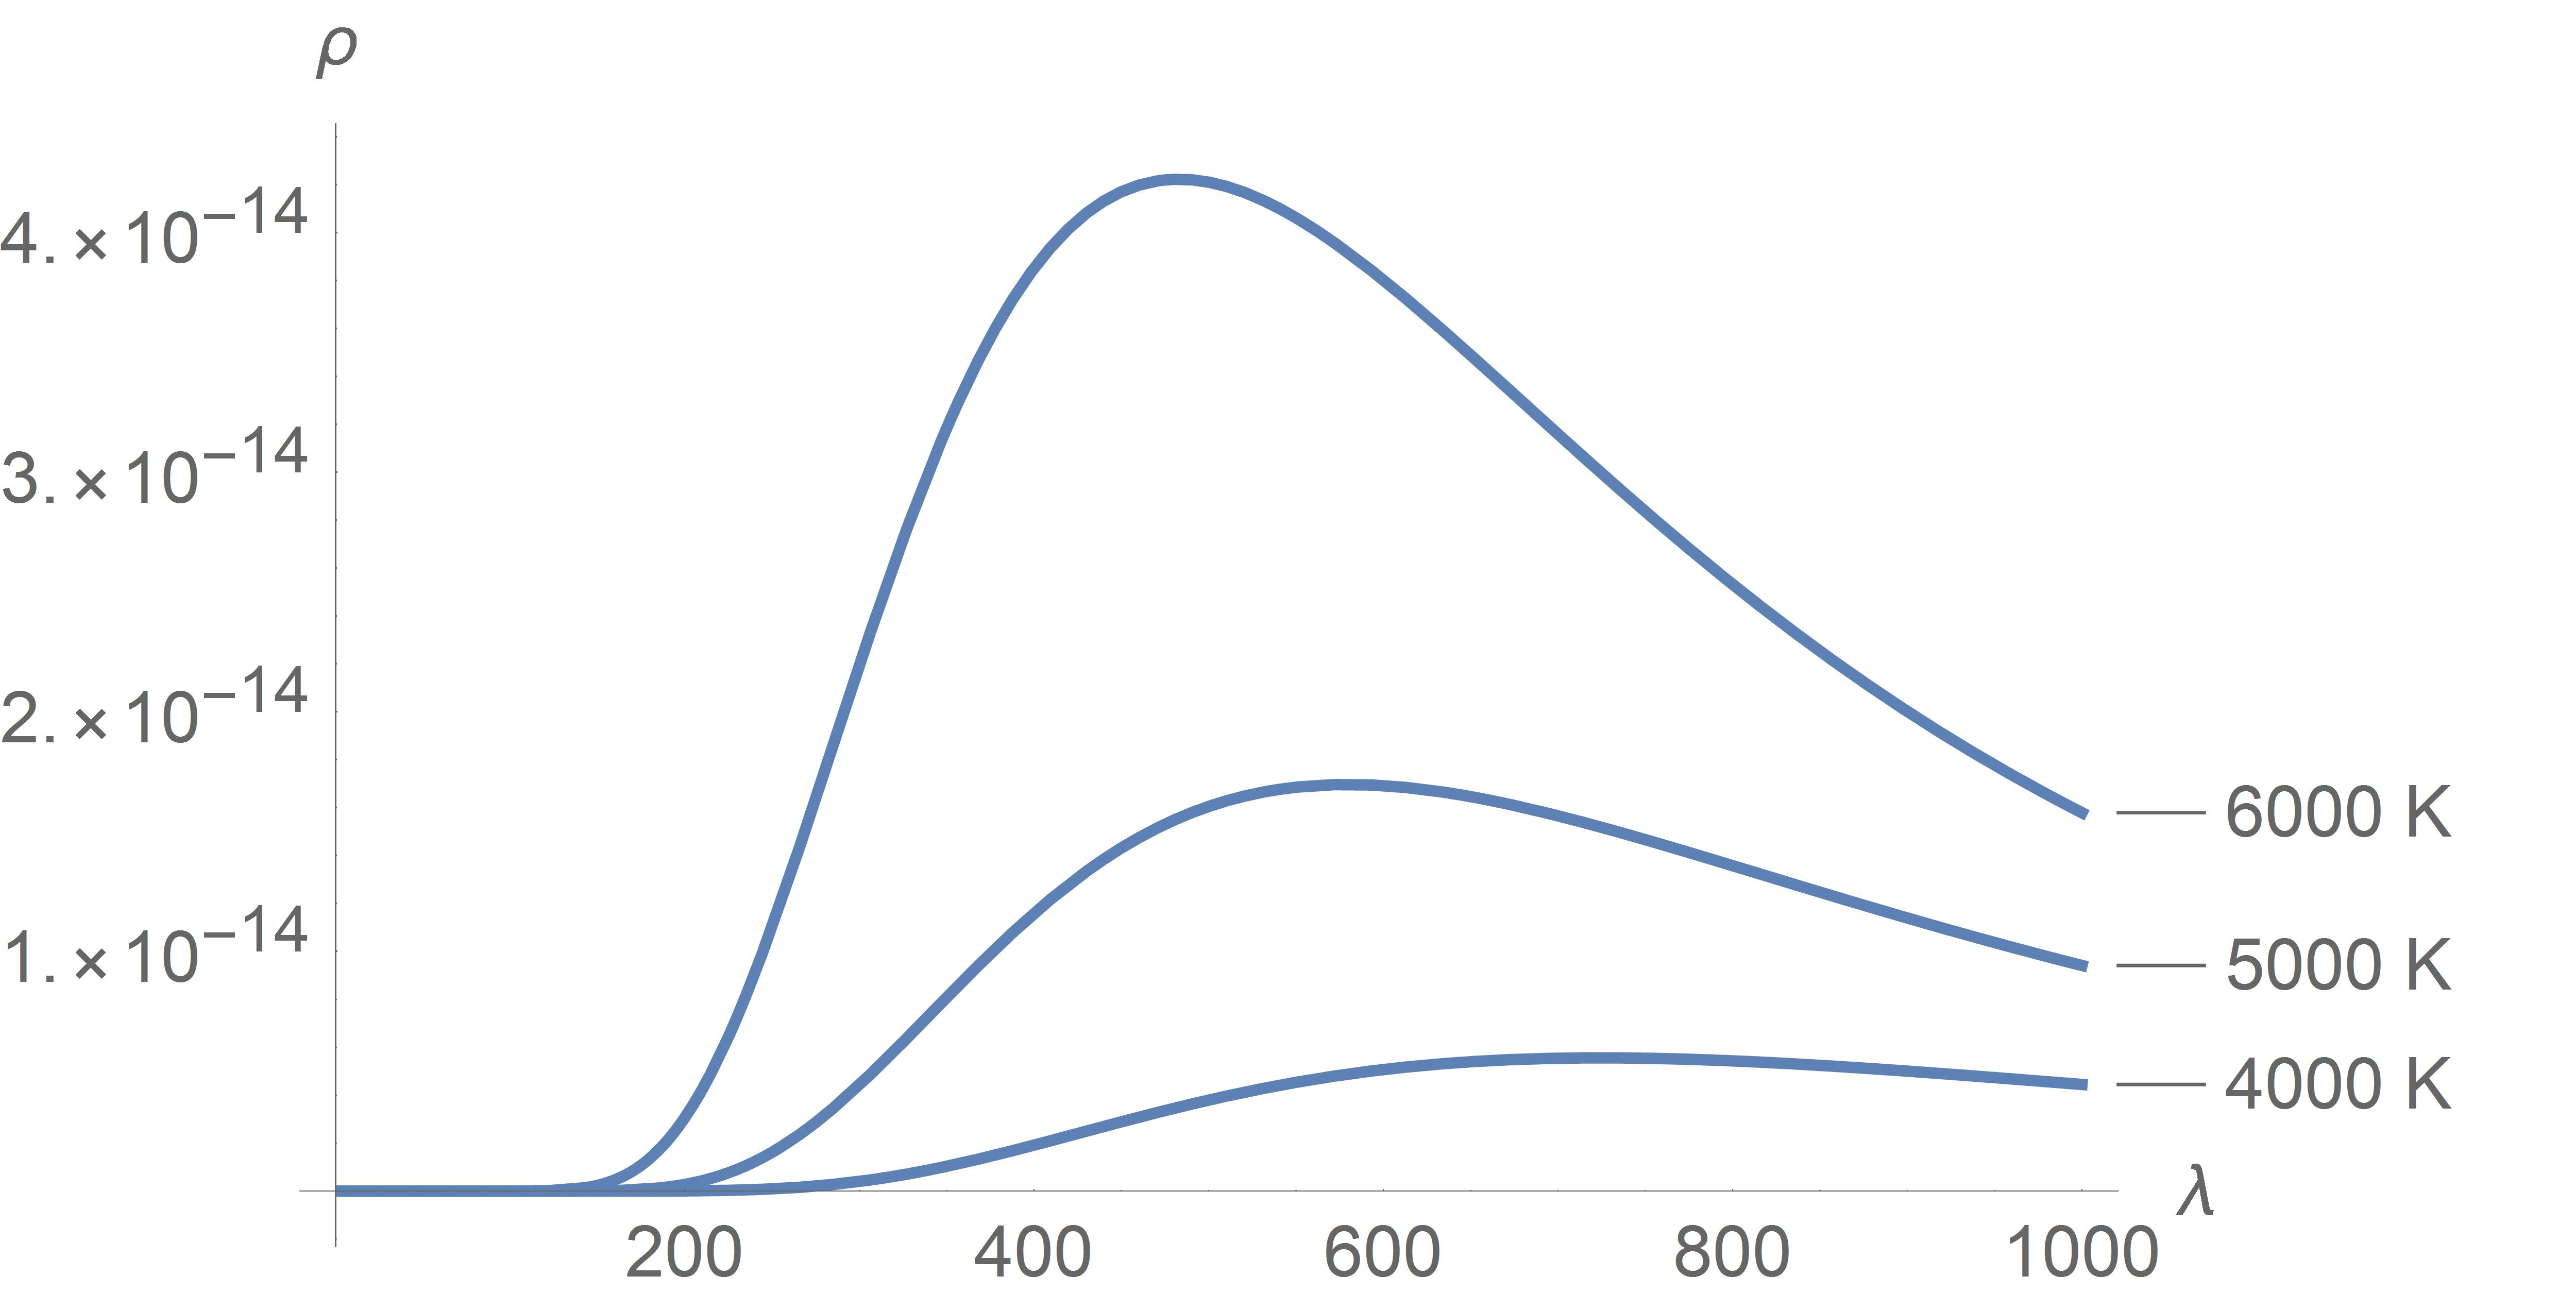
\includegraphics[width=10cm]{4000And6000Spectrum}
	\caption{Spectra for $\SI{4000}{K}$, $\SI{5000}{K}$ and $\SI{6000}{K}$}\label{fig:Prob1:4000And6000Spectrum}
\end{figure}

The mention of the surface of the sun is important for the earlier part, as different layers of the sun are at different temperatures. Some brief searching suggests that the photosphere ranges from $\SI{4000}{K}$ to $\SI{6000}{K}$. Figure \ref{fig:Prob1:4000And6000Spectrum} shows some spectra for this temperature range. The sum of these spectra (depending on the total power at each temperature for the overall scale) may probably look different than the spectrum from just one temperature.

Because of their historical importance, we also know that absorption lines are visible in the sun's spectrum. We'd expect these to show up as sharp dips in the spectrum at specific wavelengths, which would be very easily to differentiate from the blackbody spectrum.


\FloatBarrier
\lstinputlisting[
	caption=Mathematica script,
	label=lstng:Prob1:Script,
	language=Mathematica,
	backgroundcolor=\color{bggrey},
	numbers=left
]{PS3Prob1Script.m}
\FloatBarrier

\FloatBarrier
\lstinputlisting[
	caption=Mathematica output,
	label=lstng:Prob1:Output,
	backgroundcolor=\color{bggrey},
	numbers=left
]{Prob1ScriptOutput.txt}
\FloatBarrier

\end{document}
